\documentclass[12pt]{article}
\usepackage[english]{babel}
\usepackage[utf8x]{inputenc}
\usepackage[T1]{fontenc}
\usepackage{scribe}
\usepackage{listings}
\usepackage{algorithm}
\Scribe{Kriangsak Thuiprakhon}
\Lecturer{Kanat Tangwongsan}
\LectureNumber{8}
\usepackage{tikz}
\tikzset{every picture/.style={line width=0.75pt}} %set default line width to 0.75pt        
\LectureDate{DATE}
\LectureTitle{Application of Scan}
\lstset{style=mystyle}

\begin{document}
	\MakeScribeTop
\section{Paren-Matching}
Recall Paren-Matching from DS, how do we make it Parallel? Here is what we can do. let's take an example string of parenthesis:

$$(())()$$
we can assign a score to each character: say 1 to an open and -1 to a close parenthesis. we will now have an array:
$$\{1,1,-1,-1,-1,1\}$$
From here on, apply PlusScan to the collection, then the result array,A, will be:
$$A = \{\{0,1,2,1,0,1\},0\}$$   
Now we can do \textbf{map($\lambda x: x \geq 0,A$)} resulting in:
$$A' = \{T,T,T,T,T,T\}$$
Finally, we can do \textbf{reduce($\wedge, A'$)} which will give the final Boolean \textbf{T}, meaning the string has the perfect parenthesis matching.
\section{Left Copy}
Let's say there is a group of friends at the restaurant trying to order some food but not all of them actually know what to order. So, some of them will take what ever the guy on the left does. That is:
 $$O = \{a,None, b, None, None, d\}$$
To solve this problem, one can apple scan on the array $O$.  \\
$$
x*y = \begin{cases}
x &\text{if $y$ is $None$} \\
y &\text{otherwise}
\end{cases}\\
$$

We can apply $$scan(*,None,O)$$
\section{Fibonacci sequence }
\begin{definition}
the Fibonacci numbers, commonly denoted $F_n$, form a sequence, called the Fibonacci sequence, such that each number is the sum of the two preceding ones, starting from 0 and 1. That is,
$$F_0 = 0$$
$$F_1= 1$$

and 
$$F_n = F_{n-1} + F_{n-2}$$

for n > 1.
\end{definition}{}
Now, let's look at this sequence in a linear algebra point of view. That is,\\
$$
\begin{pmatrix}
1 &1 \\
1 &0
\end{pmatrix}
\begin{pmatrix}
F_{n-1} \\
F_{n-2}
\end{pmatrix}
=
\begin{pmatrix}
F_{n-1} + F_{n-2}\\
F_{n-1}
\end{pmatrix}
=\begin{pmatrix}
F_n\\
F_{n-1}
\end{pmatrix}
$$
Notice that $F_n$ can be rewritten as a some linear combination of $F_{n-1}$ and $F_{n-1}$. That is,
$$F_n = aF_{n-1} + bF_{n-2}$$
Now, if we want the n-th number of Fibonacci sequence, we can do:
$$
\begin{pmatrix}
1 &1 \\
1 &0
\end{pmatrix}
\begin{pmatrix}
1 &1 \\
1 &0
\end{pmatrix}
\begin{pmatrix}
1 &1 \\
1 &0
\end{pmatrix}
...
\underbrace{
\begin{pmatrix}
1 &1 \\
1 &0
\end{pmatrix}
}_{A}
\begin{pmatrix}
F_{n-1} \\
F_{n-2}
\end{pmatrix}
$$
now what we want looks somewhat like:
$$\{A^0, A^1,A^2, ... , \}$$
we can then apply scan as follows:
$$scan(\text{matrix multiply}, I, [A,A,A,...A]) $$
\section{List Ranking}
Let's say we have a linkedList and we want to give them some ranks (find the index of an element in Java Array). If this were to be a Java ArrayList, we could definitely call \textsc{indexOf} that return the index of element with linear time complexity. How about trying to solve it in parallel? how would one go about parallelizing this problem. In making it parallel, one can adopt \textsc{scan} function employing the technique of contraction. However, by contracting the list naively, there might be the case when a node get contracted twice with its (two) adjacent nodes. To prevent this from happening, we will go back to our old good friend, coin-flipping technique. that is to say, we will flip a coin for every node in the given LinkedList and will do contraction of two nodes if and only if the flips of the two nodes turn out to be exactly $ H \rightarrow T$, this will be discussed in more detail when we touch upon \textsc{Treecontraction} in the next lecture.  Once we have tossed a coin for every node in our list, we can then proceed with node contractions. 
In general, we can represent a LinkedList in an array as follows:
$$
    \tikzset{every picture/.style={line width=0.75pt}} %set default line width to 0.75pt        
    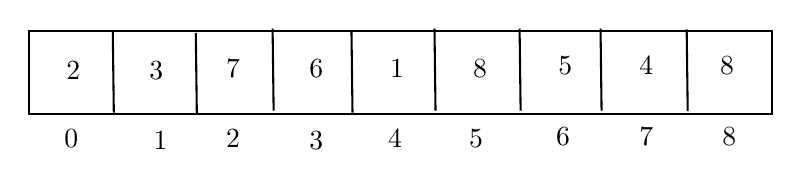
\begin{tikzpicture}[x=0.75pt,y=0.75pt,yscale=-1,xscale=1]
    %uncomment if require: \path (0,235); %set diagram left start at 0, and has height of 235
    
    %Shape: Rectangle [id:dp5783048107620253] 
    \draw   (160.5,37) -- (518.5,37) -- (518.5,77) -- (160.5,77) -- cycle ;
    %Straight Lines [id:da16291536858482958] 
    \draw    (278,36) -- (278.5,75.44) ;
    %Straight Lines [id:da07147510752614306] 
    \draw    (316,37) -- (316.5,76.44) ;
    %Straight Lines [id:da7656288099849998] 
    \draw    (356,36) -- (356.5,75.44) ;
    %Straight Lines [id:da2231965378415679] 
    \draw    (397,36) -- (397.5,75.44) ;
    %Straight Lines [id:da876762295485208] 
    \draw    (436,36) -- (436.5,75.44) ;
    %Straight Lines [id:da7355944544210964] 
    \draw    (477.5,36.28) -- (478,75.72) ;
    %Straight Lines [id:da19422431578327226] 
    \draw    (241,38) -- (241.5,77.44) ;
    %Straight Lines [id:da5119450193154419] 
    \draw    (201,37) -- (201.5,76.44) ;
    
    % Text Node
    \draw (497,54) node   [align=left] {8};
    % Text Node
    \draw (458,54) node   [align=left] {4};
    % Text Node
    \draw (419,54) node   [align=left] {5};
    % Text Node
    \draw (378,55) node   [align=left] {8};
    % Text Node
    \draw (338,55) node   [align=left] {1};
    % Text Node
    \draw (299,55) node   [align=left] {6};
    % Text Node
    \draw (259,55) node   [align=left] {7};
    % Text Node
    \draw (259,89) node   [align=left] {2};
    % Text Node
    \draw (299,90) node   [align=left] {3};
    % Text Node
    \draw (337,89) node   [align=left] {4};
    % Text Node
    \draw (376,89) node   [align=left] {5};
    % Text Node
    \draw (418,88) node   [align=left] {6};
    % Text Node
    \draw (458,88) node   [align=left] {7};
    % Text Node
    \draw (498,88) node   [align=left] {8};
    % Text Node
    \draw (224,90) node   [align=left] {1};
    % Text Node
    \draw (181,89) node   [align=left] {0};
    % Text Node
    \draw (222,56) node   [align=left] {3};
    % Text Node
    \draw (182,56) node   [align=left] {2};
    
    \end{tikzpicture}
$$

Now, we can translate the array representation to the actual LinkedList:

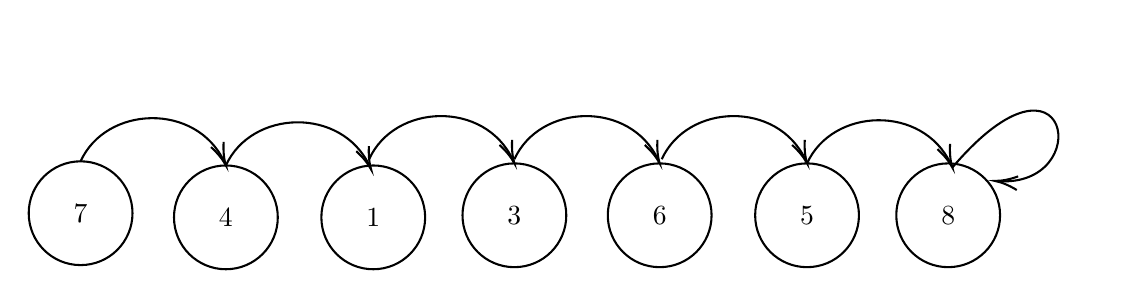
\begin{tikzpicture}[x=0.75pt,y=0.75pt,yscale=-1,xscale=1]
%uncomment if require: \path (0,235); %set diagram left start at 0, and has height of 235
%Shape: Circle [id:dp209412606148338] 
\draw   (26,63) .. controls (26,49.19) and (37.19,38) .. (51,38) .. controls (64.81,38) and (76,49.19) .. (76,63) .. controls (76,76.81) and (64.81,88) .. (51,88) .. controls (37.19,88) and (26,76.81) .. (26,63) -- cycle ;
%Shape: Circle [id:dp8786359500043003] 
\draw   (96,65) .. controls (96,51.19) and (107.19,40) .. (121,40) .. controls (134.81,40) and (146,51.19) .. (146,65) .. controls (146,78.81) and (134.81,90) .. (121,90) .. controls (107.19,90) and (96,78.81) .. (96,65) -- cycle ;
%Shape: Circle [id:dp8199816896544332] 
\draw   (167,65) .. controls (167,51.19) and (178.19,40) .. (192,40) .. controls (205.81,40) and (217,51.19) .. (217,65) .. controls (217,78.81) and (205.81,90) .. (192,90) .. controls (178.19,90) and (167,78.81) .. (167,65) -- cycle ;
%Shape: Circle [id:dp32514518330826625] 
\draw   (305,64) .. controls (305,50.19) and (316.19,39) .. (330,39) .. controls (343.81,39) and (355,50.19) .. (355,64) .. controls (355,77.81) and (343.81,89) .. (330,89) .. controls (316.19,89) and (305,77.81) .. (305,64) -- cycle ;
%Shape: Circle [id:dp9822037867033425] 
\draw   (376,64) .. controls (376,50.19) and (387.19,39) .. (401,39) .. controls (414.81,39) and (426,50.19) .. (426,64) .. controls (426,77.81) and (414.81,89) .. (401,89) .. controls (387.19,89) and (376,77.81) .. (376,64) -- cycle ;
%Shape: Circle [id:dp47504609475506554] 
\draw   (235,64) .. controls (235,50.19) and (246.19,39) .. (260,39) .. controls (273.81,39) and (285,50.19) .. (285,64) .. controls (285,77.81) and (273.81,89) .. (260,89) .. controls (246.19,89) and (235,77.81) .. (235,64) -- cycle ;
%Shape: Circle [id:dp7373998024032005] 
\draw   (444,64) .. controls (444,50.19) and (455.19,39) .. (469,39) .. controls (482.81,39) and (494,50.19) .. (494,64) .. controls (494,77.81) and (482.81,89) .. (469,89) .. controls (455.19,89) and (444,77.81) .. (444,64) -- cycle ;
%Curve Lines [id:da08360307519532739] 
\draw    (51,38) .. controls (63.25,10.99) and (106.71,9.49) .. (120.21,38.2) ;
\draw [shift={(121,40)}, rotate = 247.76] [color={rgb, 255:red, 0; green, 0; blue, 0 }  ][line width=0.75]    (10.93,-3.29) .. controls (6.95,-1.4) and (3.31,-0.3) .. (0,0) .. controls (3.31,0.3) and (6.95,1.4) .. (10.93,3.29)   ;
%Curve Lines [id:da10661682410779472] 
\draw    (121,40) .. controls (133.25,12.99) and (176.71,11.49) .. (190.21,40.2) ;
\draw [shift={(191,42)}, rotate = 247.76] [color={rgb, 255:red, 0; green, 0; blue, 0 }  ][line width=0.75]    (10.93,-3.29) .. controls (6.95,-1.4) and (3.31,-0.3) .. (0,0) .. controls (3.31,0.3) and (6.95,1.4) .. (10.93,3.29)   ;
%Curve Lines [id:da2999819680845789] 
\draw    (190,37) .. controls (202.25,9.99) and (245.71,8.49) .. (259.21,37.2) ;
\draw [shift={(260,39)}, rotate = 247.76] [color={rgb, 255:red, 0; green, 0; blue, 0 }  ][line width=0.75]    (10.93,-3.29) .. controls (6.95,-1.4) and (3.31,-0.3) .. (0,0) .. controls (3.31,0.3) and (6.95,1.4) .. (10.93,3.29)   ;
%Curve Lines [id:da9102701957834004] 
\draw    (260,37) .. controls (272.25,9.99) and (315.71,8.49) .. (329.21,37.2) ;
\draw [shift={(330,39)}, rotate = 247.76] [color={rgb, 255:red, 0; green, 0; blue, 0 }  ][line width=0.75]    (10.93,-3.29) .. controls (6.95,-1.4) and (3.31,-0.3) .. (0,0) .. controls (3.31,0.3) and (6.95,1.4) .. (10.93,3.29)   ;
%Curve Lines [id:da6050891611425984] 
\draw    (331,37) .. controls (343.25,9.99) and (386.71,8.49) .. (400.21,37.2) ;
\draw [shift={(401,39)}, rotate = 247.76] [color={rgb, 255:red, 0; green, 0; blue, 0 }  ][line width=0.75]    (10.93,-3.29) .. controls (6.95,-1.4) and (3.31,-0.3) .. (0,0) .. controls (3.31,0.3) and (6.95,1.4) .. (10.93,3.29)   ;
%Curve Lines [id:da7209329294958705] 
\draw    (401,39) .. controls (413.25,11.99) and (456.71,10.49) .. (470.21,39.2) ;
\draw [shift={(471,41)}, rotate = 247.76] [color={rgb, 255:red, 0; green, 0; blue, 0 }  ][line width=0.75]    (10.93,-3.29) .. controls (6.95,-1.4) and (3.31,-0.3) .. (0,0) .. controls (3.31,0.3) and (6.95,1.4) .. (10.93,3.29)   ;
%Curve Lines [id:da6749246461018108] 
\draw    (471,41) .. controls (527.93,-25.89) and (540.26,50.87) .. (492.95,47.56) ;
\draw [shift={(491.5,47.44)}, rotate = 365.83000000000004] [color={rgb, 255:red, 0; green, 0; blue, 0 }  ][line width=0.75]    (10.93,-3.29) .. controls (6.95,-1.4) and (3.31,-0.3) .. (0,0) .. controls (3.31,0.3) and (6.95,1.4) .. (10.93,3.29)   ;
% Text Node
\draw (469,64) node   [align=left] {8};
% Text Node
\draw (401,64) node   [align=left] {5};
% Text Node
\draw (330,64) node   [align=left] {6};
% Text Node
\draw (260,64) node   [align=left] {3};
% Text Node
\draw (192,65) node   [align=left] {1};
% Text Node
\draw (121,65) node   [align=left] {4};
% Text Node
\draw (51,63) node   [align=left] {7};
\end{tikzpicture}

Then contract the list:\\

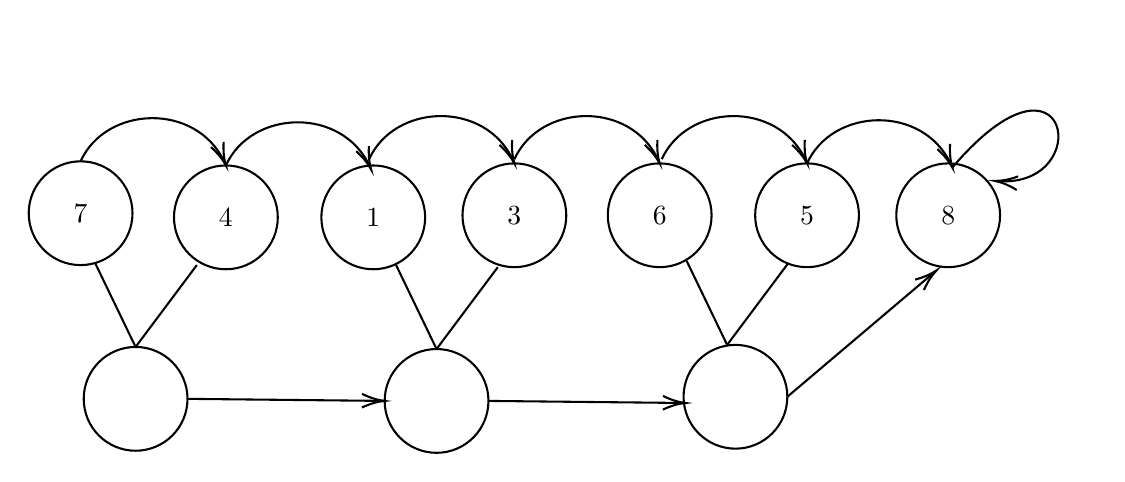
\begin{tikzpicture}[x=0.75pt,y=0.75pt,yscale=-1,xscale=1]
%uncomment if require: \path (0,235); %set diagram left start at 0, and has height of 235

%Shape: Circle [id:dp209412606148338] 
\draw   (26,63) .. controls (26,49.19) and (37.19,38) .. (51,38) .. controls (64.81,38) and (76,49.19) .. (76,63) .. controls (76,76.81) and (64.81,88) .. (51,88) .. controls (37.19,88) and (26,76.81) .. (26,63) -- cycle ;
%Shape: Circle [id:dp8786359500043003] 
\draw   (96,65) .. controls (96,51.19) and (107.19,40) .. (121,40) .. controls (134.81,40) and (146,51.19) .. (146,65) .. controls (146,78.81) and (134.81,90) .. (121,90) .. controls (107.19,90) and (96,78.81) .. (96,65) -- cycle ;
%Shape: Circle [id:dp8199816896544332] 
\draw   (167,65) .. controls (167,51.19) and (178.19,40) .. (192,40) .. controls (205.81,40) and (217,51.19) .. (217,65) .. controls (217,78.81) and (205.81,90) .. (192,90) .. controls (178.19,90) and (167,78.81) .. (167,65) -- cycle ;
%Shape: Circle [id:dp32514518330826625] 
\draw   (305,64) .. controls (305,50.19) and (316.19,39) .. (330,39) .. controls (343.81,39) and (355,50.19) .. (355,64) .. controls (355,77.81) and (343.81,89) .. (330,89) .. controls (316.19,89) and (305,77.81) .. (305,64) -- cycle ;
%Shape: Circle [id:dp9822037867033425] 
\draw   (376,64) .. controls (376,50.19) and (387.19,39) .. (401,39) .. controls (414.81,39) and (426,50.19) .. (426,64) .. controls (426,77.81) and (414.81,89) .. (401,89) .. controls (387.19,89) and (376,77.81) .. (376,64) -- cycle ;
%Shape: Circle [id:dp47504609475506554] 
\draw   (235,64) .. controls (235,50.19) and (246.19,39) .. (260,39) .. controls (273.81,39) and (285,50.19) .. (285,64) .. controls (285,77.81) and (273.81,89) .. (260,89) .. controls (246.19,89) and (235,77.81) .. (235,64) -- cycle ;
%Shape: Circle [id:dp7373998024032005] 
\draw   (444,64) .. controls (444,50.19) and (455.19,39) .. (469,39) .. controls (482.81,39) and (494,50.19) .. (494,64) .. controls (494,77.81) and (482.81,89) .. (469,89) .. controls (455.19,89) and (444,77.81) .. (444,64) -- cycle ;
%Curve Lines [id:da08360307519532739] 
\draw    (51,38) .. controls (63.25,10.99) and (106.71,9.49) .. (120.21,38.2) ;
\draw [shift={(121,40)}, rotate = 247.76] [color={rgb, 255:red, 0; green, 0; blue, 0 }  ][line width=0.75]    (10.93,-3.29) .. controls (6.95,-1.4) and (3.31,-0.3) .. (0,0) .. controls (3.31,0.3) and (6.95,1.4) .. (10.93,3.29)   ;
%Curve Lines [id:da10661682410779472] 
\draw    (121,40) .. controls (133.25,12.99) and (176.71,11.49) .. (190.21,40.2) ;
\draw [shift={(191,42)}, rotate = 247.76] [color={rgb, 255:red, 0; green, 0; blue, 0 }  ][line width=0.75]    (10.93,-3.29) .. controls (6.95,-1.4) and (3.31,-0.3) .. (0,0) .. controls (3.31,0.3) and (6.95,1.4) .. (10.93,3.29)   ;
%Curve Lines [id:da2999819680845789] 
\draw    (190,37) .. controls (202.25,9.99) and (245.71,8.49) .. (259.21,37.2) ;
\draw [shift={(260,39)}, rotate = 247.76] [color={rgb, 255:red, 0; green, 0; blue, 0 }  ][line width=0.75]    (10.93,-3.29) .. controls (6.95,-1.4) and (3.31,-0.3) .. (0,0) .. controls (3.31,0.3) and (6.95,1.4) .. (10.93,3.29)   ;
%Curve Lines [id:da9102701957834004] 
\draw    (260,37) .. controls (272.25,9.99) and (315.71,8.49) .. (329.21,37.2) ;
\draw [shift={(330,39)}, rotate = 247.76] [color={rgb, 255:red, 0; green, 0; blue, 0 }  ][line width=0.75]    (10.93,-3.29) .. controls (6.95,-1.4) and (3.31,-0.3) .. (0,0) .. controls (3.31,0.3) and (6.95,1.4) .. (10.93,3.29)   ;
%Curve Lines [id:da6050891611425984] 
\draw    (331,37) .. controls (343.25,9.99) and (386.71,8.49) .. (400.21,37.2) ;
\draw [shift={(401,39)}, rotate = 247.76] [color={rgb, 255:red, 0; green, 0; blue, 0 }  ][line width=0.75]    (10.93,-3.29) .. controls (6.95,-1.4) and (3.31,-0.3) .. (0,0) .. controls (3.31,0.3) and (6.95,1.4) .. (10.93,3.29)   ;
%Curve Lines [id:da7209329294958705] 
\draw    (401,39) .. controls (413.25,11.99) and (456.71,10.49) .. (470.21,39.2) ;
\draw [shift={(471,41)}, rotate = 247.76] [color={rgb, 255:red, 0; green, 0; blue, 0 }  ][line width=0.75]    (10.93,-3.29) .. controls (6.95,-1.4) and (3.31,-0.3) .. (0,0) .. controls (3.31,0.3) and (6.95,1.4) .. (10.93,3.29)   ;
%Curve Lines [id:da6749246461018108] 
\draw    (471,41) .. controls (527.93,-25.89) and (540.26,50.87) .. (492.95,47.56) ;
\draw [shift={(491.5,47.44)}, rotate = 365.83000000000004] [color={rgb, 255:red, 0; green, 0; blue, 0 }  ][line width=0.75]    (10.93,-3.29) .. controls (6.95,-1.4) and (3.31,-0.3) .. (0,0) .. controls (3.31,0.3) and (6.95,1.4) .. (10.93,3.29)   ;
%Straight Lines [id:da09021454387424288] 
\draw    (58,87) -- (77.5,127.44) ;
%Straight Lines [id:da1433127111995599] 
\draw    (107,88) -- (77.5,127.44) ;
%Straight Lines [id:da6502066819956911] 
\draw    (203,88) -- (222.5,128.44) ;
%Straight Lines [id:da22056480876502604] 
\draw    (252,89) -- (222.5,128.44) ;
%Straight Lines [id:da20473545330807807] 
\draw    (343,86) -- (362.5,126.44) ;
%Straight Lines [id:da18676136219017514] 
\draw    (392,87) -- (362.5,126.44) ;
%Shape: Circle [id:dp6410138198386195] 
\draw   (52.5,152.44) .. controls (52.5,138.63) and (63.69,127.44) .. (77.5,127.44) .. controls (91.31,127.44) and (102.5,138.63) .. (102.5,152.44) .. controls (102.5,166.24) and (91.31,177.44) .. (77.5,177.44) .. controls (63.69,177.44) and (52.5,166.24) .. (52.5,152.44) -- cycle ;
%Shape: Circle [id:dp843236816358602] 
\draw   (197.5,153.44) .. controls (197.5,139.63) and (208.69,128.44) .. (222.5,128.44) .. controls (236.31,128.44) and (247.5,139.63) .. (247.5,153.44) .. controls (247.5,167.24) and (236.31,178.44) .. (222.5,178.44) .. controls (208.69,178.44) and (197.5,167.24) .. (197.5,153.44) -- cycle ;
%Shape: Circle [id:dp49741461298780953] 
\draw   (341.5,151.44) .. controls (341.5,137.63) and (352.69,126.44) .. (366.5,126.44) .. controls (380.31,126.44) and (391.5,137.63) .. (391.5,151.44) .. controls (391.5,165.24) and (380.31,176.44) .. (366.5,176.44) .. controls (352.69,176.44) and (341.5,165.24) .. (341.5,151.44) -- cycle ;
%Straight Lines [id:da3260528284556792] 
\draw    (102.5,152.44) -- (195.5,153.42) ;
\draw [shift={(197.5,153.44)}, rotate = 180.6] [color={rgb, 255:red, 0; green, 0; blue, 0 }  ][line width=0.75]    (10.93,-3.29) .. controls (6.95,-1.4) and (3.31,-0.3) .. (0,0) .. controls (3.31,0.3) and (6.95,1.4) .. (10.93,3.29)   ;
%Straight Lines [id:da8703932924324034] 
\draw    (247.5,153.44) -- (340.5,154.42) ;
\draw [shift={(342.5,154.44)}, rotate = 180.6] [color={rgb, 255:red, 0; green, 0; blue, 0 }  ][line width=0.75]    (10.93,-3.29) .. controls (6.95,-1.4) and (3.31,-0.3) .. (0,0) .. controls (3.31,0.3) and (6.95,1.4) .. (10.93,3.29)   ;
%Straight Lines [id:da6262153714243609] 
\draw    (391.5,151.44) -- (461.97,91.73) ;
\draw [shift={(463.5,90.44)}, rotate = 499.73] [color={rgb, 255:red, 0; green, 0; blue, 0 }  ][line width=0.75]    (10.93,-3.29) .. controls (6.95,-1.4) and (3.31,-0.3) .. (0,0) .. controls (3.31,0.3) and (6.95,1.4) .. (10.93,3.29)   ;

% Text Node
\draw (469,64) node   [align=left] {8};
% Text Node
\draw (401,64) node   [align=left] {5};
% Text Node
\draw (330,64) node   [align=left] {6};
% Text Node
\draw (260,64) node   [align=left] {3};
% Text Node
\draw (192,65) node   [align=left] {1};
% Text Node
\draw (121,65) node   [align=left] {4};
% Text Node
\draw (51,63) node   [align=left] {7};
\end{tikzpicture}
\section{Quick Sort}
Quick sort is naturally very parallel as $Filter$ is very parallel
\section{Merge Sort}
Is Merge Sort parallel? 
Say if we halve an array
$$\{\underbrace{...}_{n/2}\underbrace{...}_{n/2}\}$$
then, the span of our mergeSort will be:
$$S(n) = S(n/2) + S_{merge}$$
The question is, what is the cost of merging two sotred arrays?
\begin{claim}
given 2 sorted sequence $A$ and $B$, there is a function, $k-th(k,A,B)$, that returns $l_A,l_B, l_A +l_B = k$ such that $A[:l_A]$ and $B[:l_B]$ are the smallest k elements of A+B done in $O(|A|+|B|)$ work, $O(log^2{(|A|+|B|))} $span
\end{claim}
This can be proven using Dual Binary Search
merge(A,B)\\
\begin{algorithm}
if len(A) =0: 
return B\\
if len(B) =0: return A \\
m=(len(A)+len(B))/2 \\
la,lb = kth(m, A,B) \\
A',B' = merge(A[:la],B[:lb]) || merge(A[la:],B[lb]:)\\
return A' +B'
\end{algorithm}


\textbf{Work and Span}

$$W(n) = W(n/2) + W(n-n/2) + O(log{n})$$
which solves to $O(n)$ where n = |A| + |B|\\

$$S(n) = S(n/2) + O(log{n})$$
which solves to $O(log^2n)$\\

Now that, $S_{merge} = O(log^2n)$,
we can go back to merge sort span analysis and complete it:
$$S_{mergeSort}(n) = S(n/2) + O(log^2n)$$
which solves to $O(log^3n)$
\end{document}